\documentclass[
  a0paper,
  portrait,
  fontscale=.35 % scales inversely (larger value=smaller font). Default is 0.292. Also affects Title etc!
  ]{baposterrptu} 

\usepackage{graphicx}             % Include Graphics
\usepackage{graphbox}	            % Alignment options for graphics
\usepackage{rptu-poster}          % some commands and color definitions
\usepackage{qrcode}               % QR Codes
\usepackage{lipsum}                % Dummy text
\usepackage{enumitem}
\usepackage{xcolor}
\usepackage{listings}
\usepackage{tcolorbox}
\usetikzlibrary{arrows.meta}

\setlist[itemize]{itemsep=.1em, topsep=.5em, leftmargin=2.5em}
%\renewcommand{\vec}[1]{\overset{\raisebox{-1ex}{$\rightarrow$}}{#1}}
\newcommand{\myvec}[1]{\vec{#1}}
\newcommand{\alt}{_\text{alt}}
\newcommand{\neu}{_\text{neu}}
\newenvironment{block}[2]
  {
    \ifstrempty{#1}{
      \begin{tcolorbox}[colback=#2!40, sharp corners, rounded corners=southeast, arc=3mm, boxrule=0mm, frame empty]
    }{
      \begin{tcolorbox}[title=#1, colbacktitle=#2, coltitle=rptuschwarz, fonttitle=\bfseries, colback=#2!40, sharp corners, rounded corners=southeast, arc=3mm, boxrule=0mm, frame empty]
    }
  }
  {
    \end{tcolorbox}
  }

%choose your poster colors here:
\colorlet{color_background}{apfel}
\colorlet{color_accents}{petrol}
% all university colors are available:
% schiefer, ozean ,nacht ,tag, petrol, pflaume, fuchsia, himbeere, mango
% ToDo: Automize pair color selection. 

\begin{document}
\begin{poster}{
    % here you can add baposter arguments to change the layout e.g. columns=3
    % this example just uses all the defaults, so no need to specify anything
    % as I know that people will complain about not enough space and try to
    % pack stuff clother, here are some example options for that
    % outercolspacing=2.5em, % adjust the white space on the left/right edges
    % boxpadding=1.5em,      % adjust the spacing within a box
    % boxheaderheight=3.5em, % change the header size
  }
  %
  {}% There used to be an top-left logo, but the current corporate design doesn't have that. 
  %
  % the poster title/Subtitle. 
  {Physik im Weltall: \\ \sf Computersimulation von Planetenbewegungen}
  %
  % the author(s)
  {angeboten von der Arbeitsgruppe Rethfeld}
  %
  % RPTU Logo top right. Replace with your own logo if required. Note that only RPTU-like Logos are permitted here.
  {\rptuLogo}
  %
  % Footer bottom left. This is supposed to hold contact details, but you can of course put anything here.
  {
    \begin{minipage}{.8\footerheight}
      \qrcode[height=.8\footerheight]{https://www.physik.uni-kl.de/rethfeld/index.php?lang=de&header_size=big}
    \end{minipage}
    \hfill
    \begin{minipage}{.35\paperwidth}
      %\textbf{License:}\\
      %Stuff like the logos are probably owned by the RPTU.\\\\
      \textbf{Kontakt:}\\
      Arbeitsgruppe für Ultrakurzzeitdynamik \\laserangeregter Festkörper
      unter Leitung von \\Prof. Bärbel Rethfeld (rethfeld@rptu.de)
    \end{minipage}
  }
  % Footer bottom right. This is supposed to hold references, but you can of course put anything here.
  {
    \begin{center}
    \includegraphics[height=\footerheight]{../programmeintrag_TdP/bild_sw.jpg}
    \end{center}
    %References:
    %\begin{itemize}
    %  \item https://github.com/Patschke/RPTU-Design
    %  \item https://rptu.de/intern/brand-portal
    %  \item https://github.com/RedHatOfficial/RedHatFont
    %  \item Original baposter by Brian Amberg
    %\end{itemize}
  }
  %
  % Your content starts from here. 
  %
  \begin{posterbox}[name=intro,column=0,row=0]{Numerische Physik}

    Warum benötigt man numerische Physik?
    \begin{itemize}
      \item Viele physikalische Probleme können nicht durch einfach lösbare Formeln beschrieben werden.
      \item Oft existiert die Formel, ist aber nicht geeignet, um die Lösung\\ schnell zu bestimmen.
    \end{itemize}
    \vspace{1em}
    Was ist numerische Physik?
    \begin{itemize}
      \item Beschreibung von Problemen durch mathematische Gleichungen 
      \item Näherungsweise Lösung der Gleichungen mit dem Computer
      \item Modifikation der Gleichungen unter Berücksichtigung\\ von experimentellen Daten
      \item Erkenntnisgewinn aus der Auswertung der computergenerierten Daten
    \end{itemize}
    \vspace{1em}
    Wo wird numerische Physik verwendet?
    \begin{itemize}
      \item Berechnung der Bahnen von Himmelskörpern und Raketen
      \item Vorhersagen von Wetter und Klimawandel
      \item Prognose von Infektionswellen während Epidemien
      \item und für noch viel mehr!
    \end{itemize}
    
  \end{posterbox}

  \begin{posterbox}[name=newton, below=intro, column=0]{Newtonsches Gravitationsgesetz}
  \begin{minipage}{.45\textwidth}
    \large
  \begin{align*}
    \myvec{F}_{12} & = G\,\frac{m_1 m_2}{|\myvec{r}_2-\myvec{r}_1|^2}\left(\myvec{r}_2-\myvec{r}_1\right)\\
    &= -\myvec{F}_{21}
  \end{align*}
  \end{minipage}\hfill
  \begin{minipage}{.45\textwidth}
    			\begin{tikzpicture}
				\coordinate (S) at (1.5,4);
				\coordinate (P) at (4.5,5.6);
				\coordinate (C) at (3, 4);
%				\draw[help lines] (0,0) grid (6,7);
				\draw[very thick, black] (3,4) ellipse (2.5 and 2.0);
				\draw[yellow!70!red, line width=3pt, -{Stealth[length=5mm]}] ($(S)!0.05!(P)$) -- ($(S)!0.4!(P)$);
				\draw[blue, line width=3pt, -{Stealth[length=5mm]}] ($(P)!0.05!(S)$) -- ($(P)!0.3!(S)$);
				\shade[ball color = yellow!80!red] (S) circle (0.5);
				\node at (S) {\color{black}\small$m_1$};
				\shade[ball color = blue] (P) circle (0.25);
				\node at (P) {\color{white}\small$m_2$};
				\draw[thick, black] (4.4,3.9) -- (4.6,4.1);
				\draw[thick, black] (4.4,4.1) -- (4.6,3.9);
				\draw[thick, black, -{Stealth[length=2mm]}] (3.3,3) -- (4.35,3.85);
				\draw[thick, black, -{Stealth[length=2mm]}] (2.7,3) -- (1.65,3.85);
				\node at (3,3) [anchor=north] {\color{black} Brennpunkte};
				\node at (1.5,4.6) [anchor=south] {\color{black} Sonne};
				\node at (4.5,6) [anchor=south] {\color{black} Planet};
				\node at (2.5, 4.9) {\color{yellow!60!red}\small $\myvec{F}_{12}$};
				\node at (3.5, 5.5) {\color{blue}\small $\myvec{F}_{21}$};
				\draw[thick, black, -{Stealth[length=2mm]}] (C) -- ($(C)!0.9!(P)$) node [midway, below, yshift=-3pt, xshift=2pt] {$\myvec{r}_{2}$};
				\draw[thick, black, -{Stealth[length=2mm]}] (C) -- ($(C)!0.8!(S)$) node [midway, below, yshift=-2pt, xshift=2pt] {$\myvec{r}_{1}$};
			\end{tikzpicture}
 
  \end{minipage}
  \vspace*{2em}
  \begin{itemize}
    \item Bereits 1687 von Isaac Newton aufgestellt
    \item Wirkt auf alle Objekte mit Masse
    \item 1. Keplersches Gesetz: Die Planeten bewegen sich auf Ellipsen, in deren einem Brennpunkt die Sonne steht
    \item Gravitationskraft eines Objekts von allen anderen Objekten abhängig \\
        $\Rightarrow$ andere Planeten ``stören'' die Bahn eines Planeten um die Sonne
    \item Entdeckung des Planeten Neptuns aufgrund von Berechnungen aus Bahnstörungen des Uranus in 1846
  \end{itemize}
  \end{posterbox}

  \begin{posterbox}[below=newton, column=0]{Euler Verfahren}
    \vspace{-.5cm}
    \begin{alignat*}{3}
      t\neu &= t\alt + \Delta t\,, && \myvec{a}_1(t\alt) &&= \frac{\myvec{F}_{12}(t\alt) + \myvec{F}_{13}(t\alt) + \dots}{m_1}\\
      \Rightarrow~~
      \myvec{v}_1(t\neu) &= \myvec{a}_1(t\alt) \cdot \Delta t + \myvec{v}_1(t)\,, ~~~~
      &&\myvec{r}_1(t\neu) &&= \myvec{v}_1(t\alt) \cdot \Delta t + \myvec{r}_1(t)
    \end{alignat*} 
    \begin{itemize}
      \item Erhöhe Zeit schrittweise um $\Delta t$.
      \item Berechne Ort und Geschwindigkeit aller Objekte zur Zeit $t + \Delta t$ aus den bereits berechneten Werten.
    \end{itemize}
  \end{posterbox}

  \begin{posterbox}[name=zeitschritt,column=1,row=0]{Der Zeitschritt}
    \begin{itemize}
      \item ist eine der wichtigsten Größen in der numerischen Beschreibung\\ dynamischer Prozesse.
      \item legt fest, wie oft Ort und Geschwindigkeit neu berechnet werden. 
      \item bestimmt Genauigkeit der Berechnung:
      \begin{itemize}
        \item kleiner Zeitschritt: gute Auflösung, lange Rechendauer
        \item grosser Zeitschritt: schlechte Auflösung, kurze Rechendauer
        \item Komplexere Lösungsverfahren erlauben größere Zeitschritte bei akzeptabler Auflösung.
      \end{itemize}
      \begin{minipage}{.45\textwidth}
      \begin{tikzpicture}[rotate=180, yscale=-1]
    %\draw[help lines] (0,0) grid (5,6);
    \draw[very thick, black] (2.5,3.5) ellipse (2 and 1);
    \draw[very thick, blue] (4.5,3.5) 
                        -- (4,4.3) 
                        -- (3.5,4.4) 
                        -- (2.5,4.6) 
                        -- (1.5,4.4) 
                        -- (1,4.3) 
                        -- (0.4,3.5)
                        -- (1,2.7) 
                        -- (1.5,2.6) 
                        -- (2.5,2.4) 
                        -- (3.5,2.6) 
                        -- (4,2.7) 
                        -- cycle;
    \draw[very thick, red] (4.5,3.5)
                        -- (3.5,4.6)
                        -- (2,4.8)
                        -- (0.5,4.2)
                        -- (0.35,3.5)
                        -- (0.6,2.9)
                    %	-- (1.3,2.9)
                        -- (2.5,2.2)
                        -- (3.5,2.4)
                        -- (4.7, 3.4)
                        -- (4.2, 4.5)
                        -- (3, 5);
\end{tikzpicture}
      \end{minipage}
      \begin{minipage}{.45\textwidth}
      Schwarz: exakte Bahn\\
      {\color{blue} Blau: passabler Zeitschritt}\\
      {\color{red} Rot: zu großer Zeitschritt}
      \end{minipage}
    \end{itemize}

  \end{posterbox}

  \begin{posterbox}[name=outlook, below=zeitschritt, column=1]{Unser Programm}
    \begin{itemize}
      \item Programmcode kann von Menschen gelesen werden.
      \item Computer können ihn verstehen und ausführen.
      \item Unser Programm besteht aus zwei Teilen: numerischer Berechnung und grafischer Oberfläche.
    \end{itemize}
    \vspace*{.75cm}
            \lstset{language=Fortran,
                    classoffset=0,
                    morekeywords={do}, keywordstyle=\color{blue!70!black},
                    classoffset=1,
                    morekeywords={sqrt, getMass, getX, getY}, keywordstyle=\color{red},
                    basicstyle=\footnotesize}
                  \textbf{Programmcode (Auszug):}
                    \begin{tcolorbox}
                \lstinputlisting{../folien/listings/programmauszug.cpp}
                    \end{tcolorbox}
                \vspace*{.75cm}
                \textbf{Grafische Oberfläche:}\\[.3cm]
                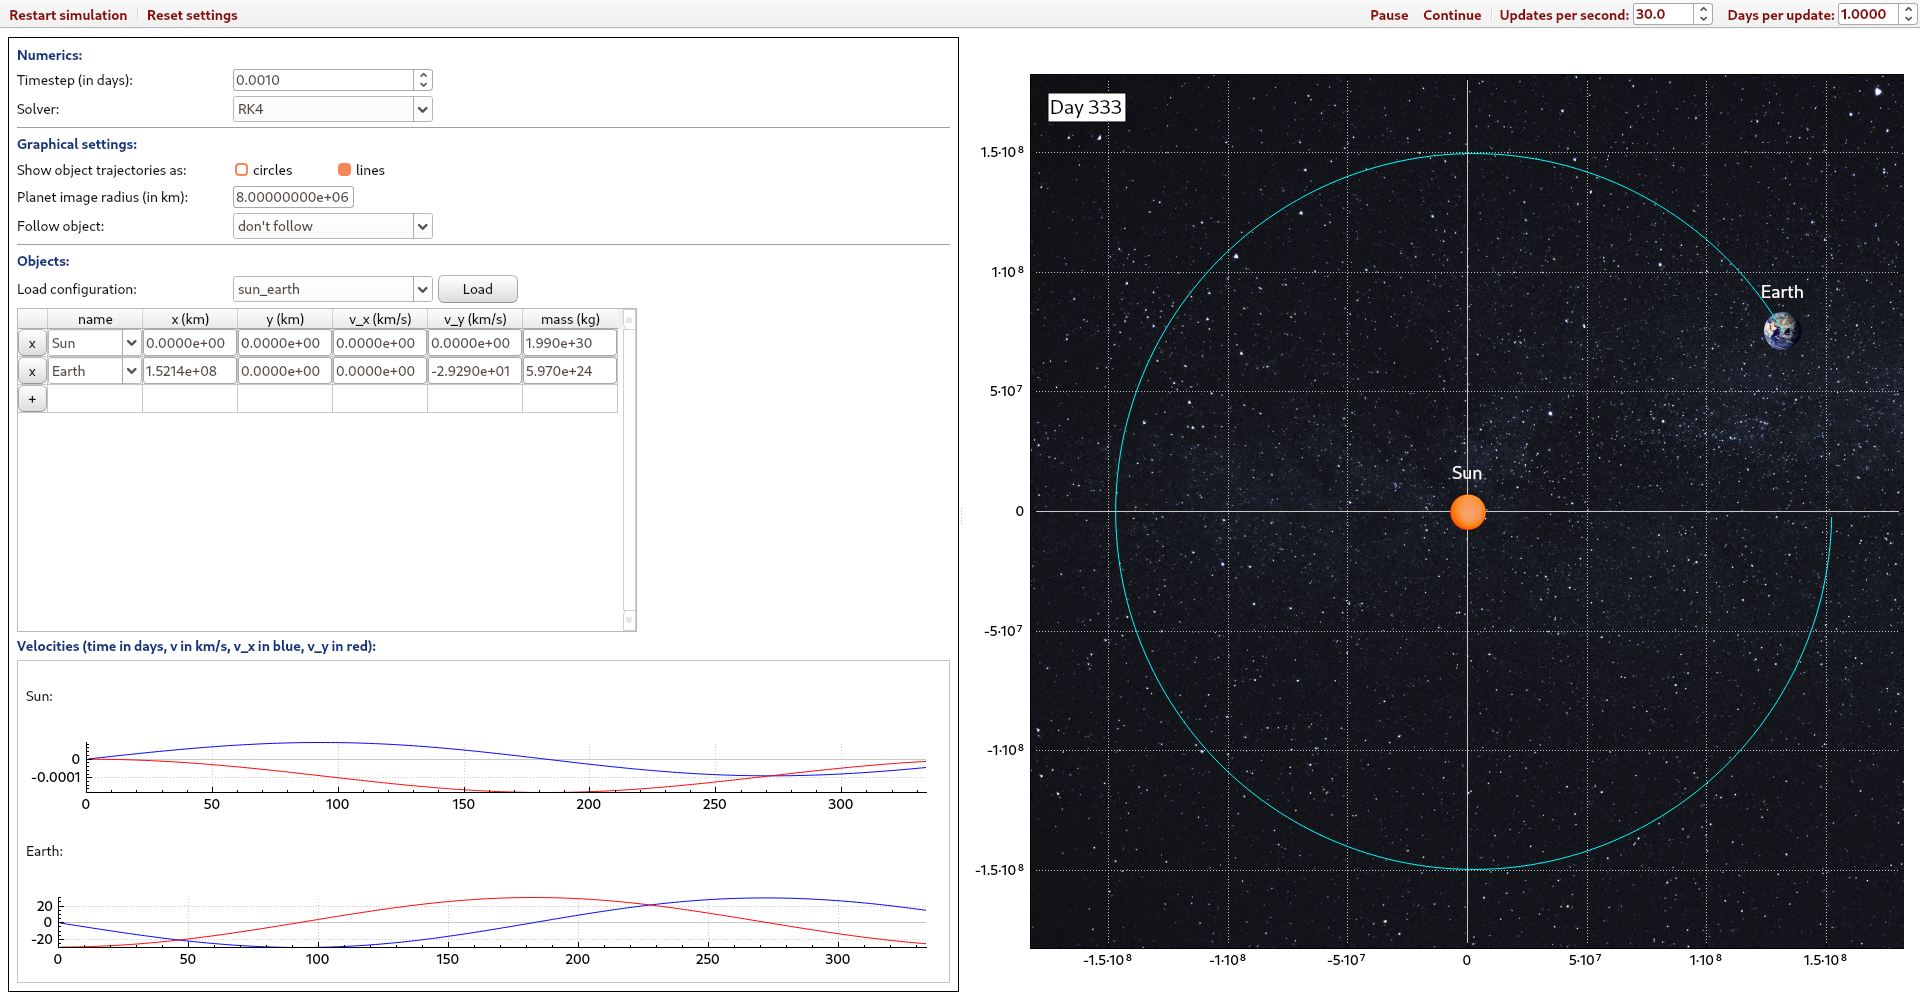
\includegraphics[width=\textwidth]{ui.png}
  \end{posterbox}

\end{poster}
\end{document}